\subsection{Part A: Null-pointer Dereference}
\subsubsection{Objectives}

\NewDocumentCommand{\cw}{v}{\texttt{\textcolor{black}{#1}}}

\begin{itemize}
    \item 熟悉 xv6 虚拟内存系统
    \item 给 xv6 添加一些现代操作系统常有的功能
\end{itemize}

\subsubsection{Steps}

\begin{enumerate}
    \item 找到原始 xv6 和 Linux 系统在访问空指针的区别
    \item 理解 xv6 如何建立页表 (page table),并且改动使其将前两页忽略 (unmapped)
    \item 改进 xv6 使其能在访问空指针的时候使用 trap 并且 kill 掉进程
\end{enumerate}

首先设置 qemu 的路径(我的安装在 root 用户下,但是实际使用另一个账户运行,所以运行指令为 \cw{sudo make qemu-nox})

\begin{textcode}
    # If the makefile can't find QEMU, specify its path here
    QEMU := /root/install/qemu-6.828-2.9.0/i386-softmmu/qemu-system-i386
\end{textcode}

编写一个程序,访问空指针,原代码见 

\cw{./user/nulldereference.c}

\begin{ccode}
    #include "types.h"
    #include "stat.h"
    #include "user.h"
        
    int main(int argc, char const *argv[])
    {
        char *a;
        printf(1, "%d\n", *a);
        exit();
    }
\end{ccode}

修改 \cw{./user/makefile.mk},添加我们编写的新程序

\begin{bashcode}
    # user programs
    USER_PROGS := \
    cat\
    echo\
    forktest\
    grep\
    init\
    kill\
    ln\
    ls\
    mkdir\
    rm\
    sh\
    stressfs\
    tester\
    usertests\
    wc\
    zombie\
    nulldereference # new program we add
\end{bashcode}

结果如下,发现指针 \cw{a} 指向未知的一串值

\begin{textcode}
    xv6...
    lapicinit: 1 0xfee00000
    cpu1: starting
    cpu0: starting
    init: starting sh
    $ nulldereference
    -115
    $ 
\end{textcode}

当我们在 \cw{Linux} 中运行类似的程序

\begin{textcode}
    zt@iZuf60n9722bkqxpt1w1sgZ:~/ECNU-OSLab/lab4/test$ ./main
    Segmentation fault
\end{textcode}

\subsubsection{page table}

32 位无符号地址被分为三个部分,第一个部分为 page directory index,第二部分为 page table index,第三部分表示 offset with page。这样每个页表构成 $2^{10}$ 个页表项,每个页表项有 $2^{12}$ 字节。然后我们也可以通过简单的位运算获取线性地址的这些部分。

回顾一下 x86 系统中使用两级树结构存放内存,每一级都是一个 1024 项的表,每一项是一个 32 位的数据,一般来说前 20 位表示物理地址的前 20 位,也就是我们要做的映射结果;后 12 位表示各种 flag。第一级存了1024个 page table,我们把这一级称为 page directory。因为每个 page table 正好有 \cw{1024x4=4096} 大,前 20 位刚好可以表示一个 page table 的头,所以这里第一级的结构里面放的都是页表。第二级存放了 1024 项 physical page number(PPN) 这 20 位替换虚拟地址中的前二十位就是物理地址了。总的来说,虚拟地址替换为物理地址的步骤时,前 10 位在 page directory 中找到 page table,然后 10 位找到 PPN,最后替换虚拟地址的前 20 位。原理如下图 \ref{fig:1} 所示

\begin{figure}[h]
    \centering
    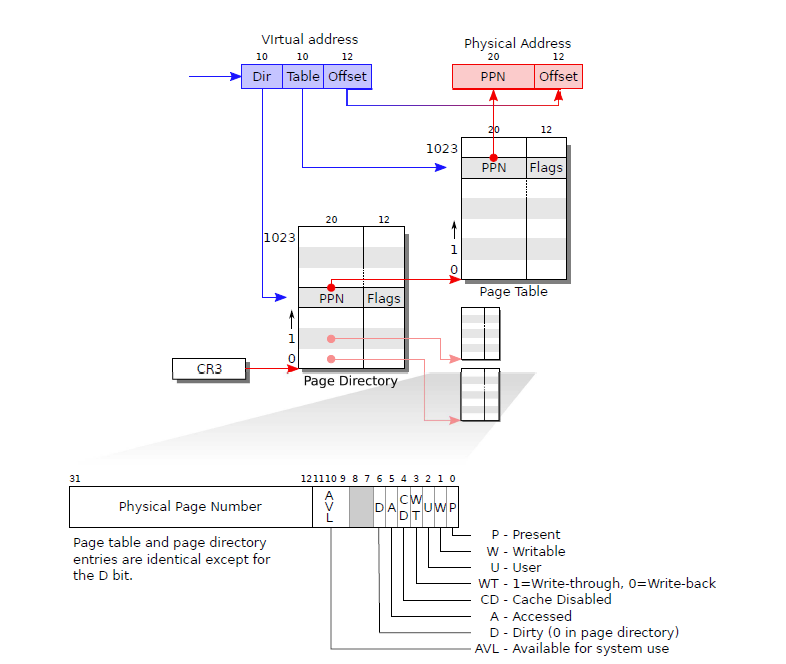
\includegraphics[width=0.8\textwidth]{img/pagemodel.PNG}
    \caption{xv6 page model}
    \label{fig:1}
\end{figure}

\cw{./kernel/mmu.h}

\begin{ccode}
    // A linear address 'la' has a three-part structure as follows:
    //
    // +--------10------+-------10-------+---------12----------+
    // | Page Directory |   Page Table   | Offset within Page  |
    // |      Index     |      Index     |                     |
    // +----------------+----------------+---------------------+
    //  \--- PDX(la) --/ \--- PTX(la) --/
        
    // page directory index
    #define PDX(la)		(((uint)(la) >> PDXSHIFT) & 0x3FF)
        
    // page table index
    #define PTX(la)		(((uint)(la) >> PTXSHIFT) & 0x3FF)
        
    // construct linear address from indexes and offset
    #define PGADDR(d, t, o)	((uint)((d) << PDXSHIFT | (t) << PTXSHIFT | (o)))
\end{ccode}

每个页表项需要一些 flag 设置他们的属性,比如说 Writeable 表示可以写入,Present 表示这个页表已经被用到了。还可以指定被当成缓存时的各种策略

\cw{./kernel/mmu.h}

\begin{ccode}
    // Page table/directory entry flags.
    #define PTE_P		0x001	// Present
    #define PTE_W		0x002	// Writeable
    #define PTE_U		0x004	// User
    #define PTE_PWT		0x008	// Write-Through
    #define PTE_PCD		0x010	// Cache-Disable
    #define PTE_A		0x020	// Accessed
    #define PTE_D		0x040	// Dirty
    #define PTE_PS		0x080	// Page Size
    #define PTE_MBZ		0x180	// Bits must be zero
\end{ccode}

\subsubsection{memory layout}

\begin{figure}[h]
    \centering
    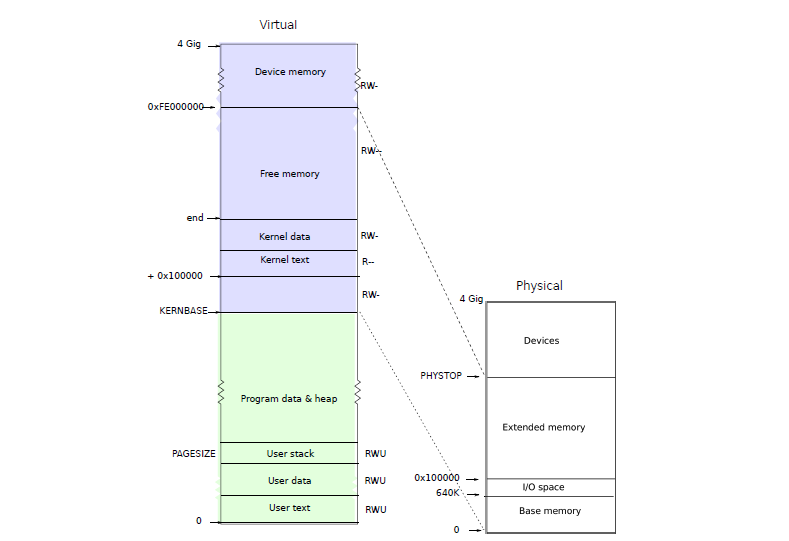
\includegraphics[width=0.8\textwidth]{img/memlayout.PNG}
    \caption{xv6 memory layout}
    \label{fig:2}
\end{figure}

用户内存从 0 开始一直到 KERNBASE。
\\ 在 \cw{./include/types.h} 中我们看到 NULL 被定义为 0。因此一个空指针会访问到 User text 部分,这部分的页表 flag 上有 \cw{Present} 因此会被认为是一个合法的内存访问。现在我们希望把前两页空出来,这样当前两页将没有 \cw{Present} flag,访问的时候 kernel 就会帮我们处理错误。

于是我们的任务主要就是:使得程序 (User text) 从 \cw{0x2000} 开始存放,留出两页的空间,涉及到的更改有:

\begin{itemize}
    \item \cw{exec} 执行程序会涉及到程序装载
    \item \cw{fork} 复制出新的进程涉及到内存复制(程序装载)
    \item \cw{userinit} 装载第一个用户程序需要特殊操作(涉及修改makefile)
    \item 修改相应的用户传入的地址的检查
\end{itemize}


\subsubsection{Code: exec}

\cw{exec} 函数首先会检查 page table directory 是否设置,以及检查 elf header。不过我们的主要关注它如何分配内存

让我们先理解一些函数(无关紧要的细节已经被忽略)

\begin{itemize}
    \item \cw{./kernel/kalloc.c kalloc} 该函数分配一个 4096 长度的物理内存空间
    \item \cw{./kernel/vm.c walkpgdir} 返回页表地址
    \item \cw{./kernel/vm.c allocuvm} 为某个进程的页表分配新的空间,从 \cw{oldsz} 增长到 \cw{newsz}
    \item \cw{./kernel/vm.c mappages} 该函数把会根据新分配的物理空间(4096长度)建立页表。也就是说会建立参数 \cw{la} (虚拟地址) 到 \cw{pa} (物理地址) 之间的映射。我们可以看到获取 \cw{la} 的地址后会检查是否该地址已经被其他物理地址占用了(\cw{panic("remap")}),否则就把 flag 加上 \cw{Present} 一起添加。由之前的定义,相邻 page table directory 本来就有相邻的地址,如果这个 page table 满了自动就会应用到下一个 page table 中。(其实也可以看作是 $2^{20}$ 个连续页表)
\end{itemize}

回到 \cw{exec} 为新程序分配内存的地方

\begin{ccode}
    sz = 0;
    for(i=0, off=elf.phoff; i<elf.phnum; i++, off+=sizeof(ph)){
        if(readi(ip, (char*)&ph, off, sizeof(ph)) != sizeof(ph))
        goto bad;
        if(ph.type != ELF_PROG_LOAD)
        continue;
        if(ph.memsz < ph.filesz)
        goto bad;
        if((sz = allocuvm(pgdir, sz, ph.va + ph.memsz)) == 0)
        goto bad;
        if(loaduvm(pgdir, (char*)ph.va, ip, ph.offset, ph.filesz) < 0)
        goto bad;
    }
    iunlockput(ip);
    ip = 0;
\end{ccode}



从 \cw{sz=0} 开始然后再执行刚刚我们提到的 \cw{allocuvm} 显然不是我们想要的结果,因为程序将从 0 开始装载而我们希望从 \cw{0x2000} 开始,这里于是有两种思路

\begin{enumerate}
    \item 更改 allocuvm 当中的 mappages,使所有的内存空间都向后位移 \cw{0x2000}
    \item 更改 exec,把程序的大小加大 \cw{0x2000}
\end{enumerate}

事实上一开始我才用前者的策略但是稍加思考后我个人偏向后者,因为 \cw{fork} 的时候会根据 \cw{proc->sz} 复制内存地址。显然改变 \cw{sz} 会使得事情简单很多,否则几乎要在每一个 \cw{mappages} 的地方都留意是否要做更改

在进程的大小处做出更改

\begin{ccode}
    // sz = 0;
    sz = 0x2000;
\end{ccode}

看起来有疑问的地方

\begin{ccode}
    if((sz = allocuvm(pgdir, sz, ph.va + ph.memsz)) == 0)
    goto bad;
\end{ccode}

我们更改了初始 \cw{sz} 的大小而没有动 \cw{ph.va, ph.memsz},那么这里分配的内存会不会发生改变?其实不会,之后我们的更改会使得所有的用户程序 \cw{sz} 都会增加保持一致性,使得这里留给程序的空间不会发生改变

用户程序的装在位置在 \cw{./user/makefile.mk} 需要被更改

\begin{bashcode}
    # location in memory where the program will be loaded
    USER_LDFLAGS += --section-start=.text=0x2000
\end{bashcode}

总之,在这一部分我们确保 \cw{exec} 执行的程序从 \cw{0x2000} 开始存放

\subsubsection{Code: fork}

\cw{fork} 函数会创建新的进程,这个过程中会复制出新的页表,这里有一个地方也需要更改

\cw{./kernel/vm.c copyuvm}

\begin{ccode}
    for(i = 0; i < sz; i += PGSIZE){
        if((pte = walkpgdir(pgdir, (void*)i, 0)) == 0)
        panic("copyuvm: pte should exist");
        if(!(*pte & PTE_P))
        panic("copyuvm: page not present");
        pa = PTE_ADDR(*pte);
        if((mem = kalloc()) == 0)
        goto bad;
        memmove(mem, (char*)pa, PGSIZE);
        if(mappages(d, (void*)i, PGSIZE, PADDR(mem), PTE_W|PTE_U) < 0)
        goto bad;
    }
\end{ccode}

在之前我们让 \cw{sz} 增大了 \cw{0x2000},因此这里复制地址看起来没什么问题,方便了许多。但是发现这里对每个在 \cw{sz} 范围内的页表项都检查了必须要有 \cw{Present} 标志,这就不是我们想要的了(前两页没有)。反正前两页我们不要,索性不复制了。这里就是第二个更改的地方

\begin{ccode}
    // for(i = 0; i < sz; i += PGSIZE){
    for (i=0x2000; i<sz; i += PGSIZE){
\end{ccode}

\subsubsection{Code: creating the first process}

第一个 user process 当然是我们的 shell 程序了,它可以在 \\
\cw{./user/init.c} 当中被找到

第一个 user process 既不是 \cw{fork} 出来的也不是某个 user process 调用 \cw{exec} 而出来的,它是手动设置的。它会先执行 \cw{initcode.S} 中的程序(这也是一个程序所以当然也要从 \cw{0x2000}开始),然后设置 trapframe 保留原始寄存器状态存放在 kernel stack 当中。从注释中我们发现,initCode 其实也是调用 \cw{exec} 执行了 init 程序。我们让 \cw{userinit} 的 eip 指向 \cw{initcode.S},设置进程状态为 RUNNABLE,然后交给 CPU 调度,准备让操作系统跑起来

于是我们要:

\begin{enumerate}
    \item 为了保留一致性我们需要更改这个手动设置的进程大小
    \item esp 位置需要更改为进程大小
    \item eip 需要指向 \cw{initcode.S} 的位置也就是 \cw{0x2000}
\end{enumerate}

\begin{ccode}
    p = allocproc();
    acquire(&ptable.lock);
    initproc = p;
    if((p->pgdir = setupkvm()) == 0)
    panic("userinit: out of memory?");
    inituvm(p->pgdir, _binary_initcode_start, (int)_binary_initcode_size);
    // p->sz = PGSIZE;
    p->sz = PGSIZE + 0x2000;
    memset(p->tf, 0, sizeof(*p->tf));
    p->tf->cs = (SEG_UCODE << 3) | DPL_USER;
    p->tf->ds = (SEG_UDATA << 3) | DPL_USER;
    p->tf->es = p->tf->ds;
    p->tf->ss = p->tf->ds;
    p->tf->eflags = FL_IF;
    // p->tf->esp = PGSIZE;
    p->tf->esp = p->sz;
    // p->tf->eip = 0;  // beginning of initcode.S
    p->tf->eip = 0x2000;
\end{ccode}

\cw{inituvm} 装载了 \cw{init} 程序,也需要更改开始位置

\begin{ccode}
    // Load the initcode into address 0 of pgdir.
    // sz must be less than a page.
    void
    inituvm(pde_t *pgdir, char *init, uint sz)
    {
    char *mem;
    
    if(sz >= PGSIZE)
        panic("inituvm: more than a page");
    mem = kalloc();
    memset(mem, 0, PGSIZE);
    // mappages(pgdir, 0, PGSIZE, PADDR(mem), PTE_W|PTE_U);
    mappages(pgdir, (void*)0x2000, PGSIZE, PADDR(mem), PTE_W|PTE_U);
    memmove(mem, init, sz);
    }
\end{ccode}

\cw{initcode} 装载在哪里得找 makefile,第四个更改的地方:

\begin{bashcode}
    initcode: kernel/initcode.o
    $(LD) $(LDFLAGS) $(KERNEL_LDFLAGS) \
        --entry=start --section-start=.text=0x2000 \
        --output=kernel/initcode.out kernel/initcode.o
    $(OBJCOPY) -S -O binary kernel/initcode.out $@
\end{bashcode}

\subsubsection{one last step}

内核需要检查用户传递过来的指针是否合法。系统调用时候内核需要用户传递的信息

系统调用从用户堆栈中获取参数。 \\
\cw{argint(), argptr(), argstr(), fetchint(), fetchstr()} 根据地址获取内容。这里我们就要更新检查地址的内容,增加如果内容来自 $[0,0x2000)$ 就会报错

\begin{ccode}
    // Fetch the int at addr from process p.
    int
    fetchint(struct proc *p, uint addr, int *ip)
    {
        if (addr < 0x2000) return -1;
        if(addr >= p->sz || addr+4 > p->sz)
            return -1;
        *ip = *(int*)(addr);
        return 0;
    }

    // Fetch the nul-terminated string at addr from process p.
    // Doesn't actually copy the string - just sets *pp to point at it.
    // Returns length of string, not including nul.
    int
    fetchstr(struct proc *p, uint addr, char **pp)
    {
        char *s, *ep;
        if (addr < 0x2000) return -1;
        if(addr >= p->sz)
            return -1;
        *pp = (char*)addr;
        ep = (char*)p->sz;
        for(s = *pp; s < ep; s++)
            if(*s == 0)
            return s - *pp;
        return -1;
    }

    int
    argptr(int n, char **pp, int size)
    {
        int i;
        
        if(argint(n, &i) < 0)
            return -1;
        if (i < 0x2000 || i >= proc->sz) return -1;
        if((uint)i >= proc->sz || (uint)i+size > proc->sz)
            return -1;
        *pp = (char*)i;
        return 0;
    }
\end{ccode}

\subsubsection{outcome}

别忘了 \cw{执行 make clean} ! makefile 对于代码没有改变的文件(比如说 \cw{init.c, initcode.S}) 不会重新编译。如果重新编译,他们还是会出现在 \cw{0x0},然后就会困惑的发现程序会在 \cw{schedule} 的时候出错 

经过一番修改后,我们运行之前的 \cw{nulldereference}

\begin{textcode}
    xv6...
    lapicinit: 1 0xfee00000
    cpu1: starting
    cpu0: starting
    init: starting sh
    $ nulldereference
    pid 3 nulldereference: trap 14 err 4 on cpu 1 eip 0x2014 addr 0x0--kill proc
    $ 
\end{textcode}

当用户程序试图访问 \cw{0x0} 时会发现那个地方的页表项没有 \cw{Present} 标记,系统会通过 \cw{trap} 退出

\subsection{Part B: Stack Rearrangement}

\subsubsection{Objectives}

\begin{enumerate}
    \item 调整进程结构,将 \cw{移到}高地址端,然后留出 \cw{5} 个 page size 大小
    \item 修改 \cw{exec, fork, userinit} 等涉及到程序进程初始化,进程复制的地方
    \item 在栈空间不够的时候修改报错为增加栈空间的大小
\end{enumerate}


\subsubsection{Code: process}

显然我们需要一个新的变量来描述系统的栈空间大小(页数)

\cw{./kernel/proc.h}

\begin{ccode}
    // Per-process state
    struct proc {
        uint sz;                     // Size of process memory (bytes)
        uint stack_sz;
        pde_t* pgdir;                // Page table
        char *kstack;                // Bottom of kernel stack for this process
        enum procstate state;        // Process state
        volatile int pid;            // Process ID
        struct proc *parent;         // Parent process
        struct trapframe *tf;        // Trap frame for current syscall
        struct context *context;     // swtch() here to run process
        void *chan;                  // If non-zero, sleeping on chan
        int killed;                  // If non-zero, have been killed
        struct file *ofile[NOFILE];  // Open files
        struct inode *cwd;           // Current directory
        char name[16];               // Process name (debugging)
    };
\end{ccode}

\subsubsection{Code: exec}

执行 \cw{exec} 的时候,是怎么初始化用户栈空间的呢?

\begin{ccode}
    // Push argument strings, prepare rest of stack in ustack.
    sp = sz;
    for(argc = 0; argv[argc]; argc++) {
        if(argc >= MAXARG)
        goto bad;
        sp -= strlen(argv[argc]) + 1;
        sp &= ~3;
        if(copyout(pgdir, sp, argv[argc], strlen(argv[argc]) + 1) < 0)
        goto bad;
        ustack[3+argc] = sp;
    }
    ustack[3+argc] = 0;

    ustack[0] = 0xffffffff;  // fake return PC
    ustack[1] = argc;
    ustack[2] = sp - (argc+1)*4;  // argv pointer

    sp -= (3+argc+1) * 4;
    if(copyout(pgdir, sp, ustack, (3+argc+1)*4) < 0)
        goto bad;
\end{ccode}

直接在 \cw{code space} 上方准备栈空间,然后将参数放进去,会对8个字节对齐。注意到这里是从地址高位开始放到地址低位,所以我们后面向地位扩展也方便了许多

于是我们要做的是:

\begin{enumerate}
    \item 更改 \cw{proc->sp} 的位置为 \cw{user top}
    \item 更改 \cw{allocuvm} 的位置从 \cw{sz, sz+PGSIZE} 到 \cw{USERTOP-PGSIZE, USERTOP}
\end{enumerate}

修改后的代码

\begin{ccode}
    int stack_sz = 0;
    // allocate one more stack at the high end of address space
    if (allocuvm(pgdir, USERTOP-stack_sz-PGSIZE, USERTOP-stack_sz) == 0)
        goto bad;
    stack_sz = PGSIZE;

    // Push argument strings, prepare rest of stack in ustack.
    sp = USERTOP;
    for(argc = 0; argv[argc]; argc++) {
        if(argc >= MAXARG)
        goto bad;
        sp -= strlen(argv[argc]) + 1;
        sp &= ~3;
        if(copyout(pgdir, sp, argv[argc], strlen(argv[argc]) + 1) < 0)
        goto bad;
        ustack[3+argc] = sp;
    }
    ustack[3+argc] = 0;

    ustack[0] = 0xffffffff;  // fake return PC
    ustack[1] = argc;
    ustack[2] = sp - (argc+1)*4;  // argv pointer

    sp -= (3+argc+1) * 4;
    if(copyout(pgdir, sp, ustack, (3+argc+1)*4) < 0)
        goto bad;

    // Save program name for debugging.
    for(last=s=path; *s; s++)
        if(*s == '/')
        last = s+1;
    safestrcpy(proc->name, last, sizeof(proc->name));

    // Commit to the user image.
    oldpgdir = proc->pgdir;
    proc->pgdir = pgdir;
    proc->sz = sz;
    proc->stack_sz = stack_sz;
    proc->tf->eip = elf.entry;  // main
    proc->tf->esp = sp;
\end{ccode}

\subsubsection{Code: fork}

我们一通修改之后,复制新进程就不仅仅是只把 \cw{0x0, proc->sz} 复制了,还需要把栈复制下来

这个时候我们需要传递一个新的参数:栈空间大小给 \cw{copyuvm},
\\ 函数定义在 \cw{defs.h}

在 \cw{copyuvm} 中新增加的代码:

\begin{ccode}
    for (i=USERTOP-stack_sz; i<USERTOP; i += PGSIZE) {
        if ((pte = walkpgdir(pgdir, (void*)i, 0)) == 0)
            panic("copyuvm: pte should exist, when copying ustack");
        if (!(*pte & PTE_P))
            panic("copyuvm: page not present, when copying ustack");
        pa = PTE_ADDR(*pte);
        if ((mem = kalloc()) == 0)
            goto bad;
        memmove(mem, (char*)pa, PGSIZE);
        if (mappages(d, (void*)i, PGSIZE, PADDR(mem), PTE_W|PTE_U) < 0)
            goto bad;
    }
\end{ccode}

更改函数定义:

\begin{ccode}
    pde_t*          copyuvm(pde_t*, uint, uint);
\end{ccode}

在 \cw{fork} 函数中的更改:

\begin{ccode}
    // Copy process state from p.
    if((np->pgdir = copyuvm(proc->pgdir, proc->sz, proc->stack_sz)) == 0){
        kfree(np->kstack);
        np->kstack = 0;
        np->state = UNUSED;
        return -1;
    }
    np->stack_sz = proc->stack_sz;
\end{ccode}

\subsubsection{Code: userinit}

像 \cw{Part A} 一样第一个用户程序 \cw{init} 也需要做出相应的修改,不过这里并没有分配 \cw{ustack} 所以我们也设置栈空间大小为 0

\begin{ccode}
    p->sz = PGSIZE + 0x2000;
    p->stack_sz = 0;
    memset(p->tf, 0, sizeof(*p->tf));
    p->tf->cs = (SEG_UCODE << 3) | DPL_USER;
    p->tf->ds = (SEG_UDATA << 3) | DPL_USER;
    p->tf->es = p->tf->ds;
    p->tf->ss = p->tf->ds;
    p->tf->eflags = FL_IF;
\end{ccode}

\subsubsection{Code: growproc}

我们需要为栈隔开 5 页的大小,因此在 \cw{growproc} 函数中留心检查


\begin{ccode}
    uint sz;
    sz = proc->sz;
    if (sz+n + 5*PGSIZE > (USERTOP - proc->stack_sz))
        return -1;
\end{ccode}

\subsubsection{system call}

相应的检查用户传入的指针的时候也需要修改,因为地址可能不只是在 $[0, sz)$ 当中了,也坑在 $[USERTOP-stack_sz, USERTOP)$ 中

\begin{ccode}
    // Fetch the int at addr from process p.
    int
    fetchint(struct proc *p, uint addr, int *ip)
    {
        if (addr < p->sz && addr+4 <= p->sz) { // below sz
            if (addr < 0x2000) return -1;
        } else if (addr >= (USERTOP - p->stack_sz)) { // in stack or above
            if (addr >= USERTOP || addr+4 > USERTOP) return -1;
        } else return -1;

        *ip = *(int*)(addr);
        return 0;
    }

    // Fetch the nul-terminated string at addr from process p.
    // Doesn't actually copy the string - just sets *pp to point at it.
    // Returns length of string, not including nul.
    int
    fetchstr(struct proc *p, uint addr, char **pp)
    {
        char *s, *ep;

        if (addr < p->sz) { // below sz
            if (addr < 0x2000) return -1;
            ep = (char*)p->sz;
        } else { // in stack or above
            if (addr >= USERTOP) return -1;
            ep = (char*)USERTOP;
        }

        if(addr >= p->sz)
            return -1;
        *pp = (char*)addr;
        
        for(s = *pp; s < ep; s++)
            if(*s == 0)
            return s - *pp;
        
        return -1;
    }
    int
    argptr(int n, char **pp, int size)
    {
        int i;
        
        if(argint(n, &i) < 0)
            return -1;
        if (i < proc->sz) {
            if (i < 0x2000) return -1;
            if (i + size > proc->sz) return -1;
        } else {
            if (i < (USERTOP - proc->stack_sz) || i >= USERTOP || i + size > USERTOP) {
                return -1;
            }
        }
        *pp = (char*)i;
        return 0;
    }
    int argstr(int n, char **pp)
    {
        int addr;
        int addr, i;
        if (argint(n, &addr) < 0)
            return -1;
        i = addr;
        if (i < proc->sz)
        {
            if (i < 0x2000)
            return -1;
            if (i + 1 > proc->sz)
            return -1;
        }
        else
        {
            if (i < (USERTOP - proc->stack_sz) || i >= USERTOP) {
            return -1;
            }
        }

        return fetchstr(proc, addr, pp);
    }
\end{ccode}

\subsubsection{Code: growstack}

接下来我们实现栈增长,按照 \cw{growproc} 的风格实现,并且在头文件也做出更改


\cw{proc.c}

\begin{ccode}
    int growstack(int n, struct proc *p) {
        uint stack_sz = p->stack_sz;
        if (USERTOP - stack_sz-n - 5*PGSIZE < p->sz)
            return -1;
        if (stack_sz+n < 0)
            return -1;
        uint newstacksz = PGROUNDUP(stack_sz+n);
        if (n > 0) {
            if (allocuvm(p->pgdir, USERTOP-newstacksz, USERTOP-stack_sz) == 0)
            return -1;
        } else if (n < 0) {
            if (deallocuvm(p->pgdir, USERTOP-stack_sz, USERTOP-newstacksz) == 0)
            return -1;
        }
        p->stack_sz = newstacksz;
        return 0;
    }
\end{ccode}

\subsubsection{Code: trap handle}
 
我们需要在检测栈空间不足时且还可以扩展栈空间的时候增加栈空间大小。由于我们并没有特判栈空间超出范围的时候是否会有问题,所以最有可能的情况就是程序访问了没有 \cw{Present} 的内存。

写一个会爆栈的程序,看报什么 \cw{trap id}

\cw{./user/stack.c}

\begin{ccode}
    #include "types.h"
    #include "stat.h"
    #include "user.h"

    int main(int argc, char const *argv[])
    {
        char a[4096];
        memset(a, 'a', sizeof(a));
        printf(1, "%s\n", a);
        exit();
    }
\end{ccode}

运行结果

\begin{textcode}
    xv6...
    lapicinit: 1 0xfee00000
    cpu1: starting
    cpu0: starting
    init: starting sh
    $ stack
    pid 3 stack: trap 14 err 6 on cpu 1 eip 0x2017 addr 0x9efc8--kill proc
    $ 
\end{textcode}

从 \cw{./kernel/defs.h} 中可以了解到这个和 nulldereference 时候一样报的是 \cw{page fault} 中断。不过可以看到现在的 \cw{addr} 为 \cw{0x9efc8} 而之前为 \cw{0x0},而 $0xA0000-0x9efc8 = 4152$ 就是爆栈的地方,我们可以根据 \cw{addr} 报出错误

\begin{ccode}
    // In user space, assume process misbehaved.
    cprintf("pid %d %s: trap %d err %d on cpu %d "
            "eip 0x%x addr 0x%x--kill proc\n",
            proc->pid, proc->name, tf->trapno, tf->err, cpu->id, tf->eip, 
            rcr2());
\end{ccode}

\cw{rcr2} 函数可以获取内存地址,我们根据他的地址判断是否是因为栈空间不够而引发页表错误,然后做出相应处理,比如增加栈空间

\begin{ccode}
    case T_PGFLT:
    {
        uint loc = rcr2(), new_stack_sz;
        cprintf("addr=%x\n", loc);
        if (loc < 0x2000 || loc < proc->sz + 0x5000 || loc >= USERTOP) {
            cprintf("we decide NOT to grow the stack!\n");
            cprintf("pid %d %s: trap %d err %d on cpu %d "
                "eip 0x%x addr 0x%x--kill proc\n",
                proc->pid, proc->name, tf->trapno, tf->err, cpu->id, tf->eip, 
                loc);
            proc->killed = 1;
            break;
        }
        new_stack_sz = USERTOP - (loc / PGSIZE * PGSIZE);
        cprintf("grow the stack from %d to %d\n", proc->stack_sz, new_stack_sz);
        growstack(new_stack_sz - proc->stack_sz, proc);  
    }
\end{ccode}

结果如图所示

\begin{textcode}
    xv6...
    lapicinit: 1 0xfee00000
    cpu1: starting
    cpu0: starting
    init: starting sh
    $ nulldereference
    addr=0
    we decide NOT to grow the stack!
    pid 3 nulldereference: trap 14 err 4 on cpu 1 eip 0x2014 addr 0x0--kill proc
    $ stack
    addr=0
    grow the stack from 4096 to 8192
    sucessful!
    $ 
\end{textcode}